%%%%%%%%%%%%%%%%%%%%%%%%%%%%%%%%%%%%%%%%%
% Original author:
% Linux and Unix Users Group at Virginia Tech Wiki 
% (https://vtluug.org/wiki/Example_LaTeX_chem_lab_report)
%
% License:
% CC BY-NC-SA 3.0 (http://creativecommons.org/licenses/by-nc-sa/3.0/)
%
%%%%%%%%%%%%%%%%%%%%%%%%%%%%%%%%%%%%%%%%%

%----------------------------------------------------------------------------------------
%	PACKAGES AND DOCUMENT CONFIGURATIONS
%----------------------------------------------------------------------------------------

\documentclass[a4paper,12pt]{article}

\usepackage{graphicx} % Required for the inclusion of images
\usepackage{titling}
\usepackage{upgreek}
\usepackage{datetime}

\setlength{\droptitle}{-8em}   % This is your set screw

\setlength\parindent{0em} % Removes all indentation from paragraphs

\renewcommand{\labelenumi}{\alph{enumi}.} % Make numbering in the enumerate environment by letter rather than number (e.g. section 6)

\usepackage{times} % Uncomment to use the Times New Roman font

%\usepackage{indentfirst}

\setlength{\parskip}{0.5em plus1pt minus1pt}

%\usepackage{showframe} % for viewing margin frames (debug)

\usepackage{fullpage}

%----------------------------------------------------------------------------------------
%	DOCUMENT INFORMATION
%----------------------------------------------------------------------------------------

\title{SDP Group 8: Final Individual Report} % Title

\author{Michael Lotkowski} % Author name

\date{\today}

\begin{document}

\maketitle % Insert the title, author and date

\begin{center}
\textbf{Mentor:} Peter Henderson
\\
\textbf{Members:} Michael Lotkowski, % Partner names
Basile Henry,
Akela Drissner,
Kostadin Kalinov,
Eugen Alpeza,
Craig Penden,
Andrew Crawford

\end{center}

%----------------------------------------------------------------------------------------
%   SECTION 1 (Introduction)
%----------------------------------------------------------------------------------------

\section{Introduction}

My contributions to our project spanned many software related topics, mostly related to the vision system. I have also helped to debug the code behind the infrared sensor and tried to incorporate a simulator, which ultimately was never used. In this brief report I will attempt to describe the overview of my contributions to the project.

%----------------------------------------------------------------------------------------
%	SECTION 2 (Communications)
%----------------------------------------------------------------------------------------

\section{Communications}

At the very begging of the project I was tasked along with Basile do design and implement a communication protocol, to allow our Python software to send and receive data from the Arduino on the robot. It was very important to us that the messages are kept very small to increase the speed and to limit the amount of data required to be resent due to packet loss. We have decided to use 8 bits per message, having the structure shown in figure \ref{fig:comms}. Where Signature is always set to 1, we have used this to make sure that we always process only our messages and not the background noise from other teams. Checksum is to check if the message is not corrupted. We set it to the number of set bits $(OPCODE ARGUMENT) \% 2$. Opcode is the command that we want the robot to execute. 1 being left motor, 2 right motor and 3 the kicker. We have used 0 as a test opcode, so that we can easily test specific parts of the code. 

Basile and I have shared the coding work on both the Arduino and Python side. We have found that this protocol worked very well and was very efficient, allowing us to design the strategy system to send lots of small commands to give us a real time control of the robot.

%----------------------------------------------------------------------------------------
%	SECTION 3 (Dot Tracking)
%----------------------------------------------------------------------------------------

\section{Colourless Dot Tracking}

The vision system which we have built upon, was using colour masks to detect different objects on the pitch. We have run into many problems with having constantly to calibrate the vision system, as otherwise we couldn't detect our robot or any other objects on the pitch. This particularly hard when changing the pitches due to extreme changes in lighting. I have decided to redesign the part of the vision system which detect the black dot on the robot's plate. The dot is fundamental to our vision system as it not only allows us to find the robot but also its orientation. 

To be able to find the dot I have used basic geometry and Gaussian filtering to sharpen the image. For each pitch that we have played on, we had to select the boundaries and zones by hand. I have designed my algorithm to search for at most 1 dot in each zone, as otherwise that would indicate that another robot illegally came into another zone. Using OpenCV I was able to get a frame containing just one zone and then apply Adaptive Gaussian filtering. At this point I would search for contours of the image. Since the dot is always a particular size and it's a circle I was able to search for contours with particular area and ones that are closest to a perfect circle. 

This method has proved accurate and reliable across different pitches and lighting conditions, without the need of calibrating the system. We have used this method of dot tracking since Milestone 2, and I believe that it has improved our vision system.

%----------------------------------------------------------------------------------------
%	SECTION 4 (Colourless Vision System)
%----------------------------------------------------------------------------------------

\section{Colourless Vision System}

After implementing the colourless dot tracking I have decided that it would be beneficial to implement a similar system for the rest of the vision system. The algorithm works by taking a square frame around the dot. During the initial attempts I have began by simply applying the same algorithm as for the dot tracking however this proved ineffective as the green plate and the green pitch weren't contrasting enough for the Adaptive Gaussian filtering. For each small frame I have applied K-means clustering for the colours, which allowed me to increase the contrast of the image. At this stage I was able to use Adaptive Gaussian Filtering and then to find contours of the image. I have applied the same philosophy as before, I have searched for contours in a particular range and ones that were the most square. 

After I have found the contour that satisfied the above constraints, I calculated the distance from the dot to the closest wall, which enabled me to know the orientation of the robot. The algorithm was nearly complete for Milestone 3 however due to performance issues we have never used it during a match. I believe with a few minor optimisations this algorithm will perform better than colour based tracking as it is independent of the lighting conditions, thus removing the need of constant calibration.

%----------------------------------------------------------------------------------------
%	SECTION 5 (Conclusion)
%----------------------------------------------------------------------------------------

\section{Conclusion}

I am pleased with my contributions, which I believe have helped the team to perform as we had. I have learnt a lot about computer vision during this course. I plan to continue developing the colourless vision system as I think it's a new approach which might prove better than the current solutions. 

%----------------------------------------------------------------------------------------
%	SECTION 6 (Appendix)
%----------------------------------------------------------------------------------------
\newpage
\section{Appendix}

\begin{figure}[ht!]
\centering
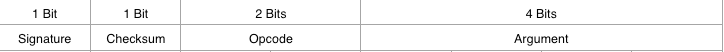
\includegraphics[width=130mm]{comms.png}
\caption{Message Structure}
\label{fig:comms}
\end{figure}

\end{document}


